% <-- a percent symbol indicates a comment which does not affect the output of LaTeX
% you can leave the preamble alone, from here ...
\documentclass[12pt]{article}

\usepackage{amssymb,amsmath,amsthm}
\usepackage{tikz}
\usepackage[top=1in, bottom=1in, left=1.25in, right=1.25in]{geometry}
\usepackage{enumitem,palatino}
\usepackage{graphicx}
\usepackage{listings}
\usepackage[colorlinks=true,citecolor=blue,linkcolor=red,urlcolor=blue]{hyperref}

\newtheorem{problem}{Problem}
\newtheorem*{theorem}{Theorem}
% ... to here

% shortcuts for blackboard bold number sets (reals, integers, etc.)
\newcommand{\II}{\ensuremath{\mathbb I}}
\newcommand{\NN}{\ensuremath{\mathbb N}}
\newcommand{\QQ}{\ensuremath{\mathbb Q}}
\newcommand{\RR}{\ensuremath{\mathbb R}}
\newcommand{\ZZ}{\ensuremath{\mathbb Z}}
\newcommand{\PP}{\ensuremath{\mathbb{P}}}

\newcommand{\eps}{\ensuremath{\epsilon}}
\newcommand{\ds}{\displaystyle}

% feel free to add more shortcuts here


\begin{document}
% replace with your name, but otherwise leave this header alone, from here ...
\small
\noindent \textsc{Math F307: Homework Assignment 7} \hfill Christopher Munoz

\normalsize
\bigskip
% ... to here
\section*{Section 6.1}

\setcounter{problem}{7}
\begin{problem}
Can a graph have an odd number of vertices of odd degree? Explain.
\begin{proof}[Solution]
  Not possible, and this is explained via the handshake lemma. If we sum up the degrees of all vertices then the resulting number is 2 multiplied by the number of edges. The number 2 multiplied by anything is by definition even.
\end{proof}
\end{problem}


\setcounter{problem}{9}
\begin{problem}
Draw a picture of the graph $G$ with $V(G) = \{x, y, z, w\}$, $E(G) = \{a, b, c, d, f, g, h\}$, and $\gamma$ given by the following table.

\begin{center}
\begin{tabular}{|c|c|c|c|c|c|c|c|}
\hline
$e$ & $a$ & $b$ & $c$ & $d$ & $f$ & $g$ & $h$ \\
\hline
$\gamma(e)$ & $\{x, y\}$ & $\{x, y\}$ & $\{w, x\}$ & $\{w, y\}$ & $\{y, z\}$ & $\{y, z\}$ & $\{w, z\}$ \\
\hline
\end{tabular}
\end{center}
\begin{proof}[Solution]
~

The graph has 4 vertices and 7 edges. Note that edges $a$ and $b$ are parallel edges between $x$ and $y$, and edges $f$ and $g$ are parallel edges between $y$ and $z$.

\begin{center}
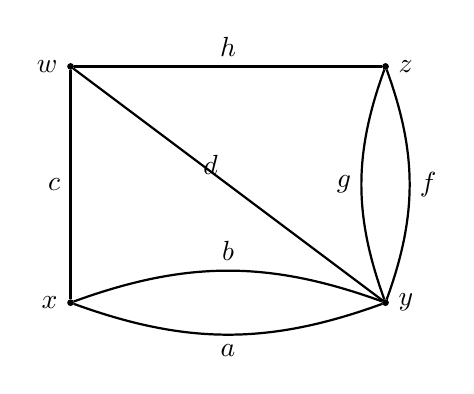
\begin{tikzpicture}[scale=2,
    vertex/.style={circle,draw,fill=black,minimum size=2pt,inner sep=0pt}]

% Vertices arranged in a square
\node[vertex,label=left:$w$] (w) at (0,1.5) {};
\node[vertex,label=left:$x$] (x) at (0,0) {};
\node[vertex,label=right:$y$] (y) at (2,0) {};
\node[vertex,label=right:$z$] (z) at (2,1.5) {};

% Edges with labels
% a and b: parallel edges between x and y
\draw[thick] (x) to[bend right=20] node[below] {$a$} (y);
\draw[thick] (x) to[bend left=20] node[above] {$b$} (y);

% c: edge between w and x
\draw[thick] (w) -- node[left] {$c$} (x);

% d: edge between w and y
\draw[thick] (w) -- node[above left] {$d$} (y);

% f and g: parallel edges between y and z
\draw[thick] (y) to[bend right=20] node[right] {$f$} (z);
\draw[thick] (y) to[bend left=20] node[left] {$g$} (z);

% h: edge between w and z
\draw[thick] (w) -- node[above] {$h$} (z);

\end{tikzpicture}
\end{center}
\end{proof}
\end{problem}




\setcounter{problem}{12}
\begin{problem}
\begin{enumerate}[label=(\alph*)]
    \item Draw pictures of all five of the regular graphs that have four vertices, each vertex of degree 2. ``All'' here means that every regular graph with four vertices and each vertex of degree 2 is isomorphic to one of the five, and no two of the five are isomorphic to each other.
\end{enumerate}

\begin{proof}[Solution]
\begin{center}
% Graph 1: C_4 (4-cycle)
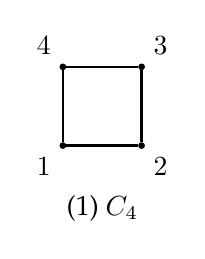
\begin{tikzpicture}[scale=1,
    vertex/.style={circle,draw,fill=black,minimum size=2pt,inner sep=0pt}]

\node[vertex,label=below left:$1$] (1) at (0,0) {};
\node[vertex,label=below right:$2$] (2) at (1,0) {};
\node[vertex,label=above right:$3$] (3) at (1,1) {};
\node[vertex,label=above left:$4$] (4) at (0,1) {};

\draw[thick] (1) -- (2);
\draw[thick] (2) -- (3);
\draw[thick] (3) -- (4);
\draw[thick] (4) -- (1);

\node at (0.5,-0.8) {(1) $C_4$};
\end{tikzpicture}
\hspace{0.5cm}
% Graph 2: Two pairs with parallel edges
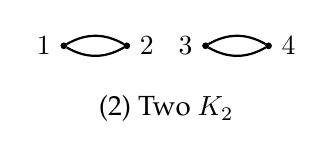
\begin{tikzpicture}[scale=1,
    vertex/.style={circle,draw,fill=black,minimum size=2pt,inner sep=0pt}]

\node[vertex,label=left:$1$] (1) at (0,0.5) {};
\node[vertex,label=right:$2$] (2) at (0.8,0.5) {};
\node[vertex,label=left:$3$] (3) at (1.8,0.5) {};
\node[vertex,label=right:$4$] (4) at (2.6,0.5) {};

\draw[thick] (1) to[bend left=30] (2);
\draw[thick] (1) to[bend right=30] (2);
\draw[thick] (3) to[bend left=30] (4);
\draw[thick] (3) to[bend right=30] (4);

\node at (1.3,-0.3) {(2) Two $K_2$};
\end{tikzpicture}
\hspace{0.5cm}
% Graph 3: Triangle + loop
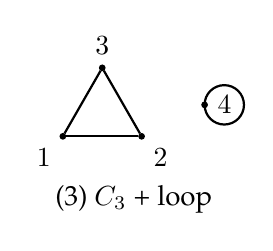
\begin{tikzpicture}[scale=1,
    vertex/.style={circle,draw,fill=black,minimum size=2pt,inner sep=0pt}]

\node[vertex,label=below left:$1$] (1) at (0,0) {};
\node[vertex,label=below right:$2$] (2) at (1,0) {};
\node[vertex,label=above:$3$] (3) at (0.5,0.87) {};
\node[vertex,label=right:$4$] (4) at (1.8,0.4) {};

\draw[thick] (1) -- (2);
\draw[thick] (2) -- (3);
\draw[thick] (3) -- (1);
\draw[thick] (4) ++ (0.25,0) circle (0.25);

\node at (0.9,-0.8) {(3) $C_3$ + loop};
\end{tikzpicture}
\hspace{0.5cm}
% Graph 4: Two loops + one doubled edge
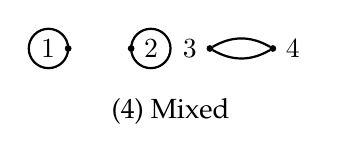
\begin{tikzpicture}[scale=1,
    vertex/.style={circle,draw,fill=black,minimum size=2pt,inner sep=0pt}]

\node[vertex,label=left:$1$] (1) at (0,0.5) {};
\node[vertex,label=right:$2$] (2) at (0.8,0.5) {};
\node[vertex,label=left:$3$] (3) at (1.8,0.5) {};
\node[vertex,label=right:$4$] (4) at (2.6,0.5) {};

\draw[thick] (1) ++ (-0.25,0) circle (0.25);
\draw[thick] (2) ++ (0.25,0) circle (0.25);
\draw[thick] (3) to[bend left=30] (4);
\draw[thick] (3) to[bend right=30] (4);

\node at (1.3,-0.3) {(4) Mixed};
\end{tikzpicture}
\hspace{0.5cm}
% Graph 5: Four loops
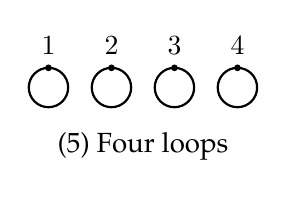
\begin{tikzpicture}[scale=1,
    vertex/.style={circle,draw,fill=black,minimum size=2pt,inner sep=0pt}]

\node[vertex,label=above:$1$] (1) at (0,0.5) {};
\node[vertex,label=above:$2$] (2) at (0.8,0.5) {};
\node[vertex,label=above:$3$] (3) at (1.6,0.5) {};
\node[vertex,label=above:$4$] (4) at (2.4,0.5) {};

\draw[thick] (1) ++ (0,-0.25) circle (0.25);
\draw[thick] (2) ++ (0,-0.25) circle (0.25);
\draw[thick] (3) ++ (0,-0.25) circle (0.25);
\draw[thick] (4) ++ (0,-0.25) circle (0.25);

\node at (1.2,-0.5) {(5) Four loops};
\end{tikzpicture}
\end{center}

\end{proof}
\end{problem}

\vspace{5in}

\setcounter{problem}{13}
\begin{problem}
\begin{enumerate}[label=(\alph*)]
    \setcounter{enumi}{1}
    \item Draw pictures of the two graphs with four vertices and four edges that have no loops or parallel edges.
\end{enumerate}
\begin{proof}[Solution]
~

With 4 vertices and 4 edges (no loops or parallel edges), there are exactly two non-isomorphic graphs:

\begin{center}
% Graph 1: C_4 (4-cycle)
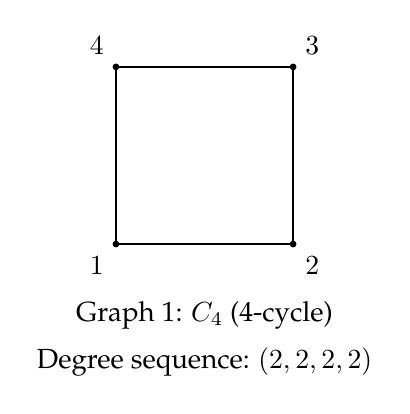
\begin{tikzpicture}[scale=1.5,
    vertex/.style={circle,draw,fill=black,minimum size=2pt,inner sep=0pt}]

\node[vertex,label=below left:$1$] (1) at (0,0) {};
\node[vertex,label=below right:$2$] (2) at (1.5,0) {};
\node[vertex,label=above right:$3$] (3) at (1.5,1.5) {};
\node[vertex,label=above left:$4$] (4) at (0,1.5) {};

\draw[thick] (1) -- (2);
\draw[thick] (2) -- (3);
\draw[thick] (3) -- (4);
\draw[thick] (4) -- (1);

\node at (0.75,-0.6) {Graph 1: $C_4$ (4-cycle)};
\node at (0.75,-1) {Degree sequence: $(2,2,2,2)$};
\end{tikzpicture}
\hspace{2cm}
% Graph 2: Triangle with tail
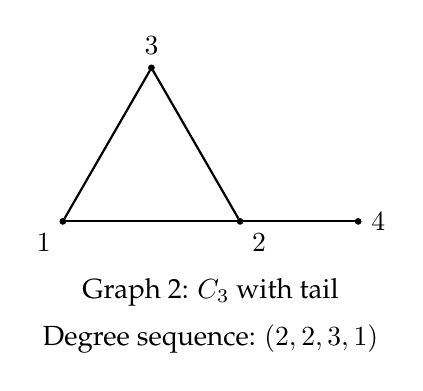
\begin{tikzpicture}[scale=1.5,
    vertex/.style={circle,draw,fill=black,minimum size=2pt,inner sep=0pt}]

\node[vertex,label=below left:$1$] (1) at (0,0) {};
\node[vertex,label=below right:$2$] (2) at (1.5,0) {};
\node[vertex,label=above:$3$] (3) at (0.75,1.3) {};
\node[vertex,label=right:$4$] (4) at (2.5,0) {};

\draw[thick] (1) -- (2);
\draw[thick] (2) -- (3);
\draw[thick] (3) -- (1);
\draw[thick] (2) -- (4);

\node at (1.25,-0.6) {Graph 2: $C_3$ with tail};
\node at (1.25,-1) {Degree sequence: $(2,2,3,1)$};
\end{tikzpicture}
\end{center}

\vspace{0.3in}

\textbf{Verification:}
\begin{itemize}
    \item Graph 1 has 4 edges forming a cycle, all vertices have degree 2
    \item Graph 2 has 3 edges forming a triangle plus 1 edge to a 4th vertex, giving degrees $(1,2,2,3)$
    \item These are the only two non-isomorphic simple graphs with 4 vertices and 4 edges
\end{itemize}

\end{proof}
\end{problem}

\vspace{3in}


\setcounter{problem}{14}
\begin{problem}
Which, if any, of the pairs of graphs shown in Figure 8 are isomorphic? Justify your answer by describing an isomorphism or explaining why one does not exist.

\begin{center}


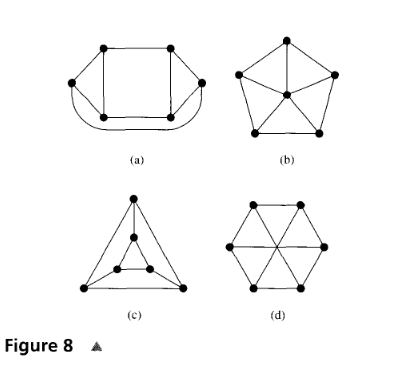
\includegraphics[width=0.8\textwidth]{figures61/figure8.png}
\end{center}
\begin{proof}[solution]
    Doesn't appear any of them are isomorphic, (a) has 2 cycles of 3 edges, and 2 cycles of 4 edges, (b) has 5 cycles of 3 edges and 1 cycle of 5 edges, (c) has 3 cycles of 4 edges and 2 cycles of 3 edges, and d 4 cycles of 4 edges and 1 of 6 edges.
\end{proof}
\end{problem}


\setcounter{problem}{15}
\begin{problem}
Describe an isomorphism between the graphs shown in Figure 9.

\begin{center}
\textbf{Figure 9:}

\vspace{0.2in}

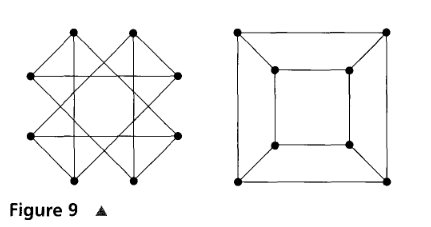
\includegraphics[width=0.6\textwidth]{figures61/figure9.png}
\end{center}
\begin{proof}[solution]
  Each vertex has 3 edges in both
  8 total vertices in both,
  There are 12 total edges in both,
  6 total cycles all of equal length(4 edges) in both,
  These are isomorphic, you can create a bijective mapping between these.
  \end{proof}
\end{problem}

\vspace{3in}

\newpage

\setcounter{problem}{19}
\begin{problem}
\begin{enumerate}[label=(\alph*)]
    \item A graph with 21 edges has seven vertices of degree 1, three of degree 2, seven of degree 3 and the rest of degree 4. How many vertices does it have?
    
    \item How would your answer to part (a) change if the graph also had six vertices of degree 0?
\end{enumerate}
\end{problem}

\begin{proof}[Solution]
~
\begin{enumerate}[label=(\alph*)]
    \item Let $k$ be the number of vertices of degree 4. By the Handshake Lemma, the sum of all degrees equals twice the number of edges:
    
    $$7(1) + 3(2) + 7(3) + k(4) = 2(21)$$
    $$7 + 6 + 21 + 4k = 42$$
    $$34 + 4k = 42$$
    $$4k = 8$$
    $$k = 2$$
    
    Total vertices: $7 + 3 + 7 + 2 = 19$ vertices.
    
    \item Vertices of degree 0 contribute nothing to the degree sum, so the calculation in part (a) remains unchanged. We still have 2 vertices of degree 4.
    
    Total vertices: $7 + 3 + 7 + 2 + 6 = 25$ vertices.
\end{enumerate}
\end{proof}

\section*{Section 6.2}

\setcounter{problem}{1}
\begin{problem}
\begin{enumerate}[label=(\alph*)]
    \item Give the vertex sequence of a simple closed path of largest possible length in the graph of Figure 7(a).
    
    \item Is your path in part (a) an Euler circuit for the graph?
\end{enumerate}

\begin{center}

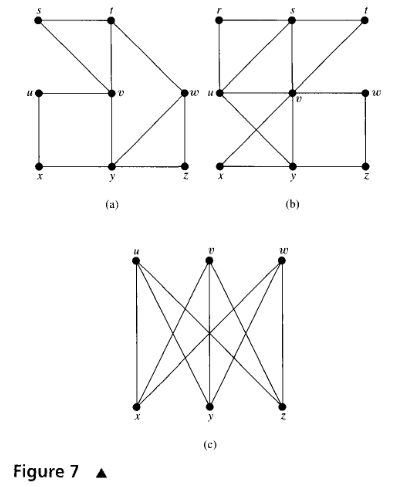
\includegraphics[width=0.4\textwidth]{figures62/figure7.png}
\end{center}
\begin{proof}[Solution] (a) [wzywtvyxuvstw] \newline
  (b) Yes, this is indeed a Euler Circuit
\end{proof}
\end{problem}

\setcounter{problem}{6}
\begin{problem}
Consider the graph shown in Figure 8(a).

\begin{enumerate}[label=(\alph*)]
    \item Describe an Euler path for this graph or explain why there isn't one.
    
    \item Describe an Euler circuit for this graph or explain why there isn't one.
\end{enumerate}

\begin{center}
\textbf{Figure 8(a):}


\includegraphics[width=0.4\textwidth]{figures62/figure8.png}
\end{center}
\begin{proof}[solution]
  (a) Eulerian path exists, just having trouble finding it. \newline
  (b) There is no Eulerian circuit since all vertices must have even degrees for this criteria and we have 2 vertices with odd degrees.
\end{proof}
\end{problem}

\setcounter{problem}{7}
\begin{problem}
Repeat Exercise 7 for the graph of Figure 8(b).

\begin{enumerate}[label=(\alph*)]
    \item Describe an Euler path for this graph or explain why there isn't one.
    
    \item Describe an Euler circuit for this graph or explain why there isn't one.
\end{enumerate}

\begin{proof}[solution]
  (a) Eulerian path does not exist, there are more than two vertices with odd degree. \newline
  (b) The lack of Eulerian path would disqualify it from having an Eulerian Circuit.
\end{proof}
\end{problem}

\setcounter{problem}{14}
\begin{problem}
An old puzzle presents a house with 5 rooms and 16 doors, as shown in Figure 9. The problem is to figure out how to walk around and through the house so as to go through each door exactly once.

\begin{enumerate}[label=(\alph*)]
    \item Is such a walk possible? Explain.
    
    \item How does your answer change if the door adjoining the two large rooms is sealed shut?
\end{enumerate}

\begin{center}
\textbf{Figure 9:}


\includegraphics[width=0.5\textwidth]{figures62/figure9.png}
\end{center}
\begin{proof}[solution]
  (a) Impossible, same problems as the 6 bridges of konigsberg, there needs to be either 0 or two nodes to create a Eulerian path. \newline
  (b)It changes the answer since now only 2 odd vertices would remain if we modlled this into a graph, meaning it would be possible.
\end{proof}
\end{problem}

\section*{Section 6.3}

\setcounter{problem}{1}
\begin{problem}
The trees in Figure 6 have seven vertices. Specify which tree in Figure 3 each is isomorphic to.

\begin{center}
\textbf{Figure 3:}


\includegraphics[width=0.6\textwidth]{figures63/figure3.png}
\end{center}

\begin{center}
\textbf{Figure 6:}


\includegraphics[width=0.4\textwidth]{figures63/figure6.png}
\end{center}
\begin{proof}[solution]
  Tree (a) in Figure 6 is isomorphic to $T_1$, Tree (b) is isomorphic to $T_5$, and Tree (c) is isomorphic to $T_11$.
\end{proof}
\end{problem}

\setcounter{problem}{5}
\begin{problem}
Find two nonisomorphic spanning trees of $K_{3,3}$ drawn in Figure 7 on page 256. Explain why they are non-isomorphic.

\begin{center}
\textbf{Figure 7 (from page 256):}

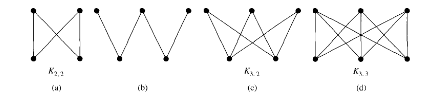
\includegraphics[width=0.5\textwidth]{figures63/k33.png}
\end{center}
\begin{proof}[Solution]
~

Two non-isomorphic spanning trees of $K_{3,3}$:

\textbf{Tree 1: Double Star}

\begin{center}
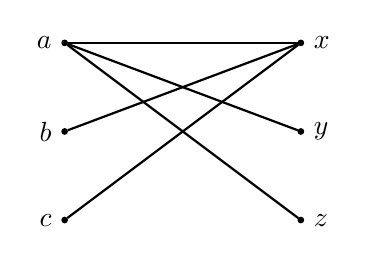
\begin{tikzpicture}[scale=1.5,
    vertex/.style={circle,draw,fill=black,minimum size=2pt,inner sep=0pt}]

% Group A vertices
\node[vertex,label=left:$a$] (a) at (0,1.5) {};
\node[vertex,label=left:$b$] (b) at (0,0.75) {};
\node[vertex,label=left:$c$] (c) at (0,0) {};

% Group B vertices
\node[vertex,label=right:$x$] (x) at (2,1.5) {};
\node[vertex,label=right:$y$] (y) at (2,0.75) {};
\node[vertex,label=right:$z$] (z) at (2,0) {};

% Spanning tree edges
\draw[thick] (a) -- (x);
\draw[thick] (a) -- (y);
\draw[thick] (a) -- (z);
\draw[thick] (b) -- (x);
\draw[thick] (c) -- (x);

\end{tikzpicture}
\end{center}

Degree sequence: $(1,1,1,1,3,3)$. Vertices $a$ and $x$ have degree 3; vertices $b,c,y,z$ are leaves.

\vspace{0.3in}

\textbf{Tree 2: Path}

\begin{center}
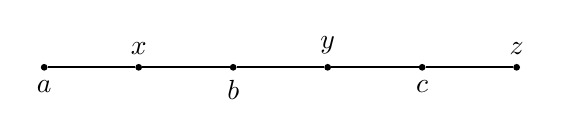
\begin{tikzpicture}[scale=1.5,
    vertex/.style={circle,draw,fill=black,minimum size=2pt,inner sep=0pt}]

% Vertices arranged in a path
\node[vertex,label=below:$a$] (a) at (0,0) {};
\node[vertex,label=above:$x$] (x) at (0.8,0) {};
\node[vertex,label=below:$b$] (b) at (1.6,0) {};
\node[vertex,label=above:$y$] (y) at (2.4,0) {};
\node[vertex,label=below:$c$] (c) at (3.2,0) {};
\node[vertex,label=above:$z$] (z) at (4,0) {};

% Path edges
\draw[thick] (a) -- (x);
\draw[thick] (x) -- (b);
\draw[thick] (b) -- (y);
\draw[thick] (y) -- (c);
\draw[thick] (c) -- (z);

\end{tikzpicture}
\end{center}

Degree sequence: $(1,1,2,2,2,2)$. Forms the path $a$-$x$-$b$-$y$-$c$-$z$.

\vspace{0.3in}

The degree sequences are different. Tree 1 has degree sequence $(1,1,1,1,3,3)$ with two vertices of degree 3, while Tree 2 has degree sequence $(1,1,2,2,2,2)$ with no vertices of degree 3. Since isomorphic graphs must have identical degree sequences, these trees are non-isomorphic.

\end{proof}
\end{problem}

\setcounter{problem}{6}
\begin{problem}
Consider a tree with $n$ vertices. It has exactly $n - 1$ edges [Lemma 2], so the sum of the degrees of its vertices is $2n - 2$ [Theorem 3 on page 230].

\begin{enumerate}[label=(\alph*)]
    \item A certain tree has two vertices of degree 4, one vertex of degree 3, and one vertex of degree 2. If the other vertices have degree 1, how many vertices are there in the graph? Hint: If the tree has $n$ vertices, $n - 4$ of them will have to have degree 1.
    
    \item Draw a tree as described in part (a).
\end{enumerate}
\end{problem}

\begin{proof}[Solution]
~
\begin{enumerate}[label=(\alph*)]
    \item Let $n$ be the total number of vertices. We have 2 vertices of degree 4, 1 of degree 3, 1 of degree 2, and the remaining $n - 4$ vertices of degree 1.
    
    The sum of degrees equals $2n - 2$:
    $$2(4) + 1(3) + 1(2) + (n-4)(1) = 2n - 2$$
    $$8 + 3 + 2 + n - 4 = 2n - 2$$
    $$9 + n = 2n - 2$$
    $$11 = n$$
    
    The tree has 11 vertices.
    
    \item 
    
    \begin{center}
    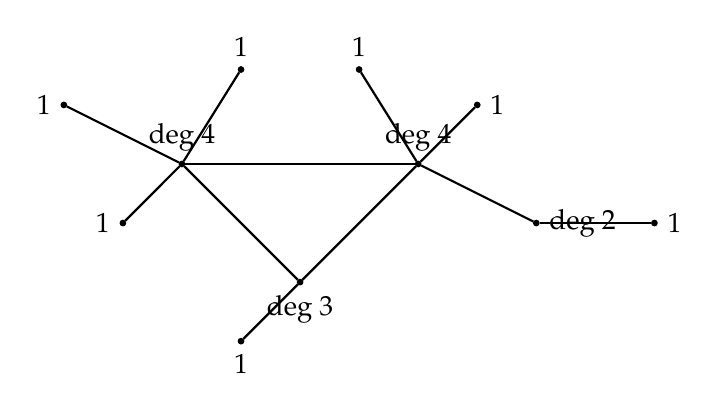
\begin{tikzpicture}[scale=1.5,
        vertex/.style={circle,draw,fill=black,minimum size=2pt,inner sep=0pt}]
    
    % Central vertices of high degree
    \node[vertex,label=above:deg 4] (v1) at (0,1) {};
    \node[vertex,label=above:deg 4] (v2) at (2,1) {};
    \node[vertex,label=below:deg 3] (v3) at (1,0) {};
    \node[vertex,label=right:deg 2] (v4) at (3,0.5) {};
    
    % Degree 1 vertices (leaves)
    \node[vertex,label=left:1] (l1) at (-1,1.5) {};
    \node[vertex,label=left:1] (l2) at (-0.5,0.5) {};
    \node[vertex,label=above:1] (l3) at (0.5,1.8) {};
    \node[vertex,label=above:1] (l4) at (1.5,1.8) {};
    \node[vertex,label=right:1] (l5) at (2.5,1.5) {};
    \node[vertex,label=below:1] (l6) at (0.5,-0.5) {};
    \node[vertex,label=right:1] (l7) at (4,0.5) {};
    
    % Edges
    \draw[thick] (v1) -- (l1);
    \draw[thick] (v1) -- (l2);
    \draw[thick] (v1) -- (l3);
    \draw[thick] (v1) -- (v3);
    
    \draw[thick] (v2) -- (l4);
    \draw[thick] (v2) -- (l5);
    \draw[thick] (v2) -- (v1);
    \draw[thick] (v2) -- (v4);
    
    \draw[thick] (v3) -- (v2);
    \draw[thick] (v3) -- (l6);
    
    \draw[thick] (v4) -- (l7);
    
    \end{tikzpicture}
    \end{center}
\end{enumerate}
\end{proof}

\setcounter{problem}{7}
\begin{problem}
Repeat Exercise 7 for a tree with two vertices of degree 5, three of degree 3, two of degree 2, and the rest of degree 1.

\begin{enumerate}[label=(\alph*)]
    \item How many vertices are there in the graph?
    
    \item Draw a tree as described.
\end{enumerate}
\end{problem}

\begin{proof}[Solution]
~
\begin{enumerate}[label=(\alph*)]
    \item Let $n$ be the total number of vertices. We have 2 vertices of degree 5, 3 of degree 3, 2 of degree 2, and the remaining $n - 7$ vertices of degree 1.
    
    The sum of degrees equals $2n - 2$:
    $$2(5) + 3(3) + 2(2) + (n-7)(1) = 2n - 2$$
    $$10 + 9 + 4 + n - 7 = 2n - 2$$
    $$16 + n = 2n - 2$$
    $$18 = n$$
    
    The tree has 18 vertices.
    
    \item 
    
    \begin{center}
    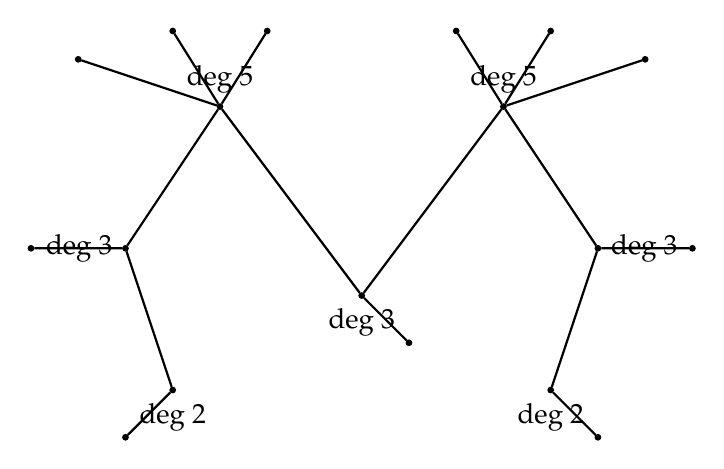
\begin{tikzpicture}[scale=1.2,
        vertex/.style={circle,draw,fill=black,minimum size=2pt,inner sep=0pt}]
    
    % Degree 5 vertices
    \node[vertex,label=above:deg 5] (v1) at (0,2) {};
    \node[vertex,label=above:deg 5] (v2) at (3,2) {};
    
    % Degree 3 vertices
    \node[vertex,label=left:deg 3] (v3) at (-1,0.5) {};
    \node[vertex,label=below:deg 3] (v4) at (1.5,0) {};
    \node[vertex,label=right:deg 3] (v5) at (4,0.5) {};
    
    % Degree 2 vertices
    \node[vertex,label=below:deg 2] (v6) at (-0.5,-1) {};
    \node[vertex,label=below:deg 2] (v7) at (3.5,-1) {};
    
    % Degree 1 vertices (11 leaves)
    \node[vertex] (l1) at (-1.5,2.5) {};
    \node[vertex] (l2) at (-0.5,2.8) {};
    \node[vertex] (l3) at (0.5,2.8) {};
    \node[vertex] (l4) at (2.5,2.8) {};
    \node[vertex] (l5) at (3.5,2.8) {};
    \node[vertex] (l6) at (4.5,2.5) {};
    \node[vertex] (l7) at (-2,0.5) {};
    \node[vertex] (l8) at (5,0.5) {};
    \node[vertex] (l9) at (2,-0.5) {};
    \node[vertex] (l10) at (-1,-1.5) {};
    \node[vertex] (l11) at (4,-1.5) {};
    
    % Edges from degree 5 vertices
    \draw[thick] (v1) -- (l1);
    \draw[thick] (v1) -- (l2);
    \draw[thick] (v1) -- (l3);
    \draw[thick] (v1) -- (v3);
    \draw[thick] (v1) -- (v4);
    
    \draw[thick] (v2) -- (l4);
    \draw[thick] (v2) -- (l5);
    \draw[thick] (v2) -- (l6);
    \draw[thick] (v2) -- (v5);
    \draw[thick] (v2) -- (v4);
    
    % Edges from degree 3 vertices
    \draw[thick] (v3) -- (l7);
    \draw[thick] (v3) -- (v6);
    
    \draw[thick] (v4) -- (l9);
    
    \draw[thick] (v5) -- (l8);
    \draw[thick] (v5) -- (v7);
    
    % Edges from degree 2 vertices
    \draw[thick] (v6) -- (l10);
    \draw[thick] (v7) -- (l11);
    
    \end{tikzpicture}
    \end{center}
\end{enumerate}
\end{proof}

\setcounter{problem}{9}
\begin{problem}
Draw pictures of the nine connected graphs with four edges and four vertices. Don't forget loops and parallel edges.
\end{problem}

\begin{proof}[Solution]
~

The nine connected graphs with 4 vertices and 4 edges are:

\begin{center}
% Graph 1: C_4
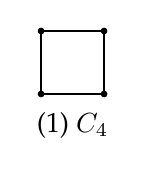
\begin{tikzpicture}[scale=0.8,
    vertex/.style={circle,draw,fill=black,minimum size=2pt,inner sep=0pt}]
\node[vertex] (1) at (0,0) {};
\node[vertex] (2) at (1,0) {};
\node[vertex] (3) at (1,1) {};
\node[vertex] (4) at (0,1) {};
\draw[thick] (1) -- (2) -- (3) -- (4) -- (1);
\node at (0.5,-0.5) {(1) $C_4$};
\end{tikzpicture}
\hspace{0.4cm}
% Graph 2: Triangle with tail
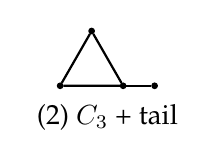
\begin{tikzpicture}[scale=0.8,
    vertex/.style={circle,draw,fill=black,minimum size=2pt,inner sep=0pt}]
\node[vertex] (1) at (0,0) {};
\node[vertex] (2) at (1,0) {};
\node[vertex] (3) at (0.5,0.87) {};
\node[vertex] (4) at (1.5,0) {};
\draw[thick] (1) -- (2) -- (3) -- (1);
\draw[thick] (2) -- (4);
\node at (0.75,-0.5) {(2) $C_3$ + tail};
\end{tikzpicture}
\hspace{0.4cm}
% Graph 3: Path with parallel edge
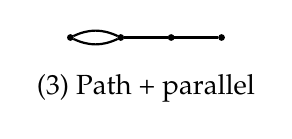
\begin{tikzpicture}[scale=0.8,
    vertex/.style={circle,draw,fill=black,minimum size=2pt,inner sep=0pt}]
\node[vertex] (1) at (0,0.5) {};
\node[vertex] (2) at (0.8,0.5) {};
\node[vertex] (3) at (1.6,0.5) {};
\node[vertex] (4) at (2.4,0.5) {};
\draw[thick] (1) to[bend left=25] (2);
\draw[thick] (1) to[bend right=25] (2);
\draw[thick] (2) -- (3);
\draw[thick] (3) -- (4);
\node at (1.2,-0.3) {(3) Path + parallel};
\end{tikzpicture}
\hspace{0.4cm}
% Graph 4: Star with parallel edge
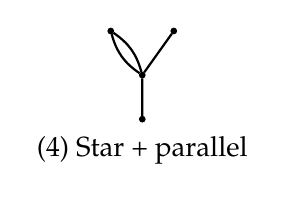
\begin{tikzpicture}[scale=0.8,
    vertex/.style={circle,draw,fill=black,minimum size=2pt,inner sep=0pt}]
\node[vertex] (c) at (0.5,0.5) {};
\node[vertex] (1) at (0,1.2) {};
\node[vertex] (2) at (1,1.2) {};
\node[vertex] (3) at (0.5,-0.2) {};
\draw[thick] (c) to[bend left=20] (1);
\draw[thick] (c) to[bend right=20] (1);
\draw[thick] (c) -- (2);
\draw[thick] (c) -- (3);
\node at (0.5,-0.7) {(4) Star + parallel};
\end{tikzpicture}
\hspace{0.4cm}
% Graph 5: 2 parallel + 1 edge
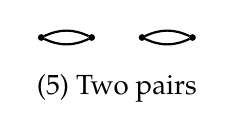
\begin{tikzpicture}[scale=0.8,
    vertex/.style={circle,draw,fill=black,minimum size=2pt,inner sep=0pt}]
\node[vertex] (1) at (0,0.5) {};
\node[vertex] (2) at (0.8,0.5) {};
\node[vertex] (3) at (1.6,0.5) {};
\node[vertex] (4) at (2.4,0.5) {};
\draw[thick] (1) to[bend left=25] (2);
\draw[thick] (1) to[bend right=25] (2);
\draw[thick] (3) to[bend left=25] (4);
\draw[thick] (3) to[bend right=25] (4);
\node at (1.2,-0.3) {(5) Two pairs};
\end{tikzpicture}

\vspace{0.5cm}

% Graph 6: Triangle with loop
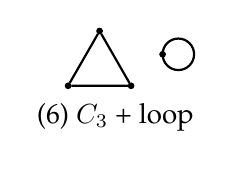
\begin{tikzpicture}[scale=0.8,
    vertex/.style={circle,draw,fill=black,minimum size=2pt,inner sep=0pt}]
\node[vertex] (1) at (0,0) {};
\node[vertex] (2) at (1,0) {};
\node[vertex] (3) at (0.5,0.87) {};
\node[vertex] (4) at (1.5,0.5) {};
\draw[thick] (1) -- (2) -- (3) -- (1);
\draw[thick] (4) ++ (0.25,0) circle (0.25);
\node at (0.75,-0.5) {(6) $C_3$ + loop};
\end{tikzpicture}
\hspace{0.4cm}
% Graph 7: Path with loop
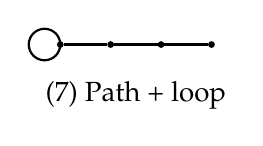
\begin{tikzpicture}[scale=0.8,
    vertex/.style={circle,draw,fill=black,minimum size=2pt,inner sep=0pt}]
\node[vertex] (1) at (0,0.5) {};
\node[vertex] (2) at (0.8,0.5) {};
\node[vertex] (3) at (1.6,0.5) {};
\node[vertex] (4) at (2.4,0.5) {};
\draw[thick] (1) -- (2);
\draw[thick] (2) -- (3);
\draw[thick] (3) -- (4);
\draw[thick] (1) ++ (-0.25,0) circle (0.25);
\node at (1.2,-0.3) {(7) Path + loop};
\end{tikzpicture}
\hspace{0.4cm}
% Graph 8: Star with loop
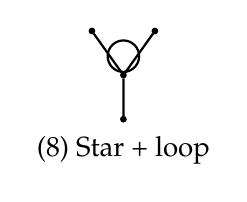
\begin{tikzpicture}[scale=0.8,
    vertex/.style={circle,draw,fill=black,minimum size=2pt,inner sep=0pt}]
\node[vertex] (c) at (0.5,0.5) {};
\node[vertex] (1) at (0,1.2) {};
\node[vertex] (2) at (1,1.2) {};
\node[vertex] (3) at (0.5,-0.2) {};
\draw[thick] (c) -- (1);
\draw[thick] (c) -- (2);
\draw[thick] (c) -- (3);
\draw[thick] (c) ++ (0,0.3) circle (0.25);
\node at (0.5,-0.7) {(8) Star + loop};
\end{tikzpicture}
\hspace{0.4cm}
% Graph 9: Edge + 2 loops
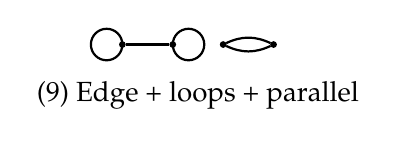
\begin{tikzpicture}[scale=0.8,
    vertex/.style={circle,draw,fill=black,minimum size=2pt,inner sep=0pt}]
\node[vertex] (1) at (0,0.5) {};
\node[vertex] (2) at (0.8,0.5) {};
\node[vertex] (3) at (1.6,0.5) {};
\node[vertex] (4) at (2.4,0.5) {};
\draw[thick] (1) -- (2);
\draw[thick] (1) ++ (-0.25,0) circle (0.25);
\draw[thick] (2) ++ (0.25,0) circle (0.25);
\draw[thick] (3) to[bend left=25] (4);
\draw[thick] (3) to[bend right=25] (4);
\node at (1.2,-0.3) {(9) Edge + loops + parallel};
\end{tikzpicture}
\end{center}

\end{proof}

\setcounter{problem}{10}
\begin{problem}
\begin{enumerate}[label=(\alph*)]
    \item Show that a forest with $n$ vertices and $m$ components has $n - m$ edges.
\end{enumerate}
\end{problem}

\begin{proof}[Solution]
~
\begin{enumerate}[label=(\alph*)]
    \item A forest is a disjoint union of trees. Let the $m$ components be trees $T_1, T_2, \ldots, T_m$ with $n_1, n_2, \ldots, n_m$ vertices respectively.
    
    Since each tree $T_i$ has $n_i$ vertices, it has exactly $n_i - 1$ edges (by Lemma 2).
    
    The total number of vertices is:
    $$n = n_1 + n_2 + \cdots + n_m$$
    
    The total number of edges is:
    $$e = (n_1 - 1) + (n_2 - 1) + \cdots + (n_m - 1)$$
    $$e = (n_1 + n_2 + \cdots + n_m) - m$$
    $$e = n - m$$
    
    Therefore, a forest with $n$ vertices and $m$ components has $n - m$ edges.
\end{enumerate}
\end{proof}


\end{document}
